\chapter{Iniciación}
\noindent En el presente capítulo se pretende describir el caso de estudio, los requerimientos funcionales, casos de uso y aspectos tecnicos.

\noindent El objetivo de esta fase en el Proceso Unificado Ágil, es obtener una máxima compresión cliente - equipo de desarrollo. Los requerimientos funcionales, el alcance del software a desarrollar (criterios de aceptación).

\section {Visión General - Caso de estudio}
\noindent Las empresas que ofrecen servicio de pedidos a domicilio a través de motorizados (mototaxis) en su mayor parte administran su negocio por medio de archivos Excel por lo cual tienen muchas limitaciones.
Para conocer el negocio y las respectivas actividades que realizan, se entrevistó a dos empresas de este rubro (Scooters, Ser). El flujo de trabajo desde que les llega el pedido consiste en:
\begin{itemize}
\item El encargo de recibir los pedidos, por cada pedido que llega, comunica a todos los motorizados por radio frecuencia.
\item Cada empresa tiene parqueos en los diferentes negocios de comidas en la mayoría y de acuerdo al orden de llegada tiene prioridad para que sean asignados a ese pedido.
\item En la mayor parte se tiene el siguiente caso para asignar un pedido. El pedido llega de algún restaurante o negocio de comidas o de cliente directo que quiere el pedido. Por decir, el restaurante de donde se debe recoger el pedido, la empresa de mototaxis no tiene parqueo por lo cual se debe ir preguntando quién quiere tomar el pedido, entonces los motorizados se reportan y dan su ubicación y si están disponibles y se ponen de acuerdo entre ellos quién podría tomar el pedido ya que se puede tener más de dos motorizados que quieran tomar ese pedido.
\end{itemize}
\indent Entre otras actividades administrativas dentro de las empresas de mototaxis:
\begin{itemize}
\item Cada motorizado debe pagar diariamente un monto por frecuencia recibida. en el transcurso del día deben reportarse en su central para iniciar su trabajo.
\item La empresa establece una multa diaria por inasistencia a todos los motorizados y se les recarga al momento que se reportan.
\item Al final del día (entre la 12:00 am), el encargado de la central realiza su informe de ingresos por frecuencia, cobro de multas y motorizados que no asistieron a trabajar.
\end{itemize}
\section{Identificación de requerimientos}
\noindent La identificación de requerimientos se basará en las actividades que realizan las empresas del rubro de servicios en mototaxis contemplando los siguientes escenarios principales para el desarrollo de la aplicación web (Software como un servicio - SaaS):
\begin{itemize}
\item \textbf{Administración de Pedidos}: Los operadores deben poder registrar los pedidos realizados por los clientes y asignar al motorizado que le corresponde.
\item \textbf {Administración de Mototaxis}: Los operadores deberán poder registrar, actualizar información o deshabilitar a los respectivos motorizados de la empresa. También podrán registrar el pago por frecuencia diaria o las multas por inasistencia.  
\item \textbf{Administración de usuarios}: Cada Empresa de mototaxis solo podrá tener una cuenta administrador y  varias cuentas de operadores.
\item \textbf{Administración de Seguridad}: El acceso a la información y las diferentes operaciones que puedan realizar los usuarios deberán ser controlados bajo perfiles de usuarios (administrador de la empresa y operadores).
\end{itemize}

\section{Requerimientos funcionales}

\noindent Los requerimientos funcionales fueron agrupados de acuerdo a las áreas de administración detectadas en común en las empresas y también se consideró la definición de la administración de seguridad que tiene que ver más con la aplicación web.

\begin{table}[H]
	\centering
    \begin{tabular}{ |c|p{10cm}|c| }
	  \hline
	  \rowcolor{indigo-dark} \multicolumn{3}{|c|}{ \textcolor{white}{\textbf{Administración de Pedidos}}} \\
	  \hline
	  \rowcolor{indigo-light} \textbf{N\#} & \centering \textbf{Descripción} & \textbf{Prioridad} \\
	  \hline
	  1 & El usuario con perfil de operador podrá registrar los pedidos realizados por los clientes. & Alta\\
	  \hline
	  2 & El usuario con perfil de operador tendrá la opción de poder consultar a qué mototaxi corresponde la asignación del pedido. & Media \\
	  \hline
	  3 & El usuario con perfil de operador podrá ver la lista de pedidos realizados en el dia.   & Baja \\
	  \hline
	\end{tabular}
	\caption{Requerimientos de la administración de pedidos}
\end{table}

\begin{table}[H]
	\centering
    \begin{tabular}{ |c|p{10cm}|c| }
	  \hline
	  \rowcolor{indigo-dark} \multicolumn{3}{|c|}{ \textcolor{white}{\textbf{Administración de Mototaxis}}} \\
	  \hline
	  \rowcolor{indigo-light} \textbf{N\#} & \centering \textbf{Descripción} & \textbf{Prioridad} \\
	  \hline
	  1 & El usuario con perfil de operador podrá registrar nuevos motorizados a la respectiva empresa a la cual corresponde. & Alta \\
	  \hline
	  2 & El usuario con perfil de operador podrá registrar el cobro por frecuencia diaria realizada a los respectivos mototaxis. & Alta \\
	  \hline
	  3 & El usuario con perfil de operador podrá registrar el cobro por multa de inasistencia a los respectivos motorizados de la empresa. & Alta \\
	  \hline
	  4 & El usuario con perfil de operador podrá listar los mototaxis correspondientes a la empresa & Baja \\
	  \hline
	\end{tabular}
	\caption{Requerimientos de la Administración de Mototaxis de las respectivas empresas}
\end{table}

\begin{table}[H]
	\centering
    \begin{tabular}{ |c|p{10cm}|c| }
	  \hline
	  \rowcolor{indigo-dark} \multicolumn{3}{|c|}{ \textcolor{white}{\textbf{Administración de Usuarios}}} \\
	  \hline
	  \rowcolor{indigo-light} \textbf{N\#} & \centering \textbf{Descripción} & \textbf{Prioridad} \\
	  \hline
	  1 & El usuario con perfil de administrador es el único que puede crear cuentas de operadores para la empresa correspondiente. & Alta\\
	  \hline
	  2 & El usuario con perfil de administrador solo podrá ver la información relacionada a los operadores de la empresa, ingresos diarios y mensuales por cobro por frecuencia y multas por inasistencia de los mototaxis. & Media \\
	  \hline
	  3 & La aplicación web deberá proporcionar la opción que los usuarios puedan  cambiar sus datos personales. & Baja \\
	  \hline
	\end{tabular}
	\caption{Requerimientos de los perfiles de usuarios para las empresas}
\end{table}

\begin{table}[H]
	\centering
    \begin{tabular}{ |c|p{10cm}|c| }
	  \hline
	  \rowcolor{indigo-dark} \multicolumn{3}{|c|}{ \textcolor{white}{\textbf{Administración de Seguridad}}} \\
	  \hline
	  \rowcolor{indigo-light} \textbf{N\#} & \centering \textbf{Descripción} & \textbf{Prioridad} \\
	  \hline
	  1 & La aplicación web deberá controlar el acceso a la información a través de la autentificación de usuarios y mostrará el menú de operaciones que puede realizar el usuario de acuerdo al perfil de usuario (Administrador u Operador). & Alta\\
	  \hline
	  2 & La aplicación web deberá controlar las operaciones de acuerdo al tipo de perfil  de usuario que define por cada operación en los recursos de información con los accesos de (lectura, escritura, eliminación y/o actualización). & Alta\\
	  \hline
	  3 & La aplicación web deberá controlar el acceso a la información a los diferentes usuarios que solo puedan ingresar a la información de la empresa a la cual pertenecen. & Alta \\
	  \hline
	  4 & La aplicación web deberá permitir crear una cuenta empresa en conjunto con la cuenta administrador. & Media \\
	  \hline
	  5 & La aplicación web deberá proporcionar las opciones de iniciar sesión y cerrar session. &  Media\\
	  \hline
	  6 & La aplicación web deberá permitir a los usuarios cambiar contraseña. &  Baja \\
	  \hline
	\end{tabular}
	\caption{Requerimientos de Seguridad de la aplicación web}
\end{table}

\section{Perfiles de usuarios}
\noindent La aplicación web define dos tipos de perfiles de usuarios (Administrador y Operador). Cada perfil de  usuario puede realizar cierto número de operaciones dentro la aplicación web.
\noindent los perfiles de usuarios definidos son:
\begin{itemize}
\item \textbf{Administrador}: El perfil de administrador es creado al mismo tiempo cuando se crea la cuenta de la empresa en la aplicación web. Este perfil de usuario está enfocado a administrar las cuentas de los operadores correspondientes a la empresa, reportes de ingresos por cobro de frecuencia y multas y ver los respectivos mototaxis registrados.
\begin{figure}[ht]
  \centering
  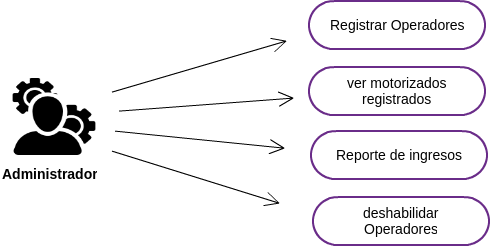
\includegraphics[width=8cm, height=4cm]{chapter3-admin-profile.png}
  \caption{Acciones que puede realizar un Administrador [Elaboracion propia ]}  
\end{figure}
\item \textbf{Operador}: El perfil de Operador está enfocado a registrar nuevos motorizados, registrar pago de frecuencias y multas. Este perfil de usuario está enfocado a al registro de las diferentes transacciones o actividades diarias que se realizan en la empresa.
\begin{figure}[ht]
  \centering
  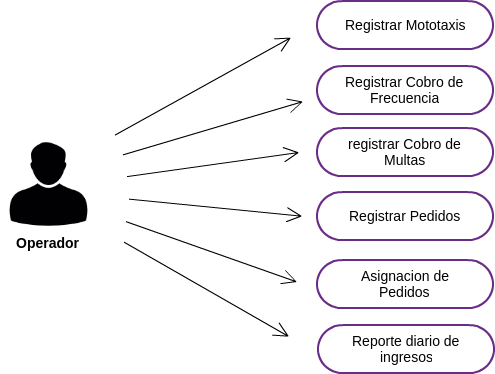
\includegraphics[width=8cm, height=7cm]{chapter3-operator-profile.png}
  \caption{Acciones que puede realizar un Operador [Elaboracion propia ]}  
\end{figure}
\end{itemize}
\section{Requerimientos no funcionales}
\section{Viabilidad Técnica y Económica}
\section{Arquitectura del Sistema}
\section{Planificación del Sistema a desarrollar}

